\section{II - Fonction d'activation}
\begin{frame}{II - Fonction d'activation}
\begin{block}{Fonction d'activation}
Sans l'utilisation de la fonction d'activation, le neurone est multilinéaire par rapport à ses entrées, il n'est donc pas capable que de faire des régressions linéaires sur les données d'entrées. \\
Les fonctions d'activation permettent donc une classification non linéaire.
\end{block}
\end{frame}


\begin{frame}{II - Fonction d'activation}
\begin{figure}
	\begin{subfigure}[]{0.3\textwidth}
		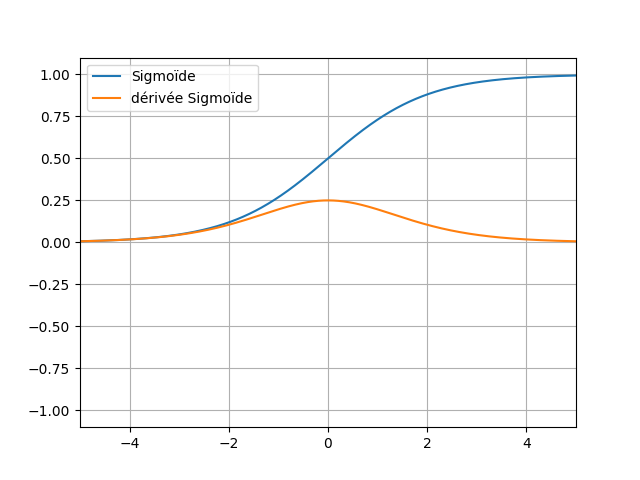
\includegraphics[width=90px]{0-Sigmoide.png}
  		\caption{Sigmoïde}
	\end{subfigure}
	\begin{subfigure}[]{0.3\textwidth}
		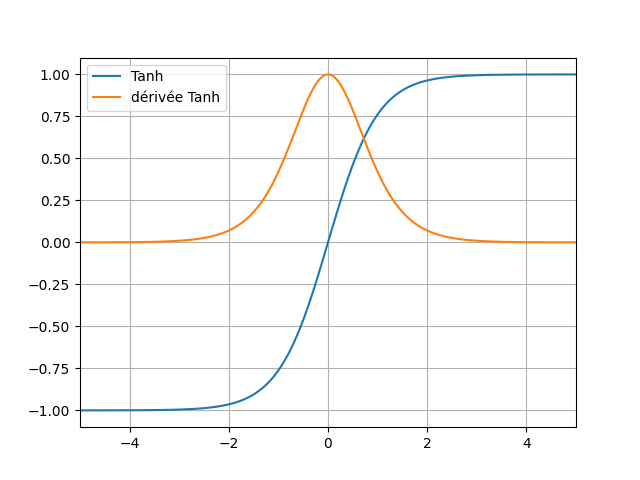
\includegraphics[width=90px]{0-Tanh.png}
  		\caption{Tanh}
	\end{subfigure}
	\begin{subfigure}[]{0.3\textwidth}
		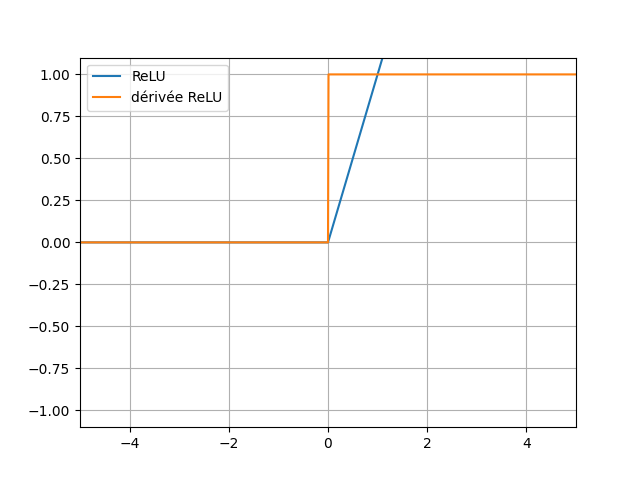
\includegraphics[width=90px]{0-ReLU.png}
		\caption{ReLU}
	\end{subfigure}
\end{figure}

\begin{block}{}
\centering
\begin{tabular}{ l || c | c | }
   Fonction & Formule & Dérivée \\ \hline \\
   Sigmoïde (a) & $\mathlarger{\frac{1}{1+e^{-x}}}$ & $f(x) \times (1-f(x))$ \\ \\
   Tangente Hyperbolique (Tanh) (b) & $\mathlarger{\frac{e^{x}-e^{-x}}{e^{x}+e^{-x}}}$ & $1-f(x)^2$ \\ \\
   Unité Linéaire Rectifiée (ReLU) (c) & $max(0, x)$ & $ \left\{\begin{array}{ll}
      														  0 & \mbox{si } x<0 \\
     														  1 & \mbox{sinon }   \end{array}\right.$ \\
\end{tabular}
\end{block}
\end{frame}

\begin{frame}{II - Fonction d'activation, les spécificités}


\begin{block}{}
\centering
\begin{tabular}{ |p{0.15\textwidth}||p{0.35\textwidth}|p{0.35\textwidth} | }
\hline 
   Fonction & Avantage & Inconvénient \\ [20pt] \hline \hline 
   Sigmoïde & A valeur dans $]0, 1[$ ce qui facilite les classifications binaires & Dérivée petite vers $\pm\infty$, il y a peu d'apprentissage pour ces valeurs \\ [20pt] \hline
   Tanh & Utilisé dans les couches cachées car fonction impaire  & Même problème que la Sigmoïde \\ [20pt] \hline
   ReLU & Plus simple à calculer, prend en compte le gradient pour toute valeur positive & Dérivée nulle en x négatif ce qui peut rendre des neurones inutiles \\ [20pt] \hline 
\end{tabular}
\end{block}
\end{frame}
